%%\documentclass[a4paper,12pt,oneside]{llncs}
\documentclass[12pt,letterpaper]{article}
\usepackage[right=2cm,left=3cm,top=2cm,bottom=2cm,headsep=0cm]{geometry}

%%%%%%%%%%%%%%%%%%%%%%%%%%%%%%%%%%%%%%%%%%%%%%%%%%%%%%%%%%%
%% Juego de caracteres usado en el archivo fuente: UTF-8
\usepackage{ucs}
\usepackage[utf8x]{inputenc}

%%%%%%%%%%%%%%%%%%%%%%%%%%%%%%%%%%%%%%%%%%%%%%%%%%%%%%%%%%%
%% Juego de caracteres usado en la salida dvi
%% Otra posibilidad: \usepackage{t1enc}
\usepackage[T1]{fontenc}

%%%%%%%%%%%%%%%%%%%%%%%%%%%%%%%%%%%%%%%%%%%%%%%%%%%%%%%%%%%
%% Ajusta maergenes para a4
%\usepackage{a4wide}

%%%%%%%%%%%%%%%%%%%%%%%%%%%%%%%%%%%%%%%%%%%%%%%%%%%%%%%%%%%
%% Uso fuente postscript times, para que los ps y pdf queden y pequeños...
\usepackage{times}

%%%%%%%%%%%%%%%%%%%%%%%%%%%%%%%%%%%%%%%%%%%%%%%%%%%%%%%%%%%
%% Posibilidad de hipertexto (especialmente en pdf)
%\usepackage{hyperref}
\usepackage[bookmarks = true, colorlinks=true, linkcolor = black, citecolor = black, menucolor = black, urlcolor = black]{hyperref}

%%%%%%%%%%%%%%%%%%%%%%%%%%%%%%%%%%%%%%%%%%%%%%%%%%%%%%%%%%%
%% Graficos 
\usepackage{graphics,graphicx}

%%%%%%%%%%%%%%%%%%%%%%%%%%%%%%%%%%%%%%%%%%%%%%%%%%%%%%%%%%%
%% Ciertos caracteres "raros"...
\usepackage{latexsym}

%%%%%%%%%%%%%%%%%%%%%%%%%%%%%%%%%%%%%%%%%%%%%%%%%%%%%%%%%%%
%% Matematicas aun más fuertes (american math dociety)
\usepackage{amsmath}

%%%%%%%%%%%%%%%%%%%%%%%%%%%%%%%%%%%%%%%%%%%%%%%%%%%%%%%%%%%
\usepackage{multirow} % para las tablas
\usepackage[spanish,es-tabla]{babel}

%%%%%%%%%%%%%%%%%%%%%%%%%%%%%%%%%%%%%%%%%%%%%%%%%%%%%%%%%%%
%% Fuentes matematicas lo mas compatibles posibles con postscript (times)
%% (Esto no funciona para todos los simbolos pero reduce mucho el tamaño del
%% pdf si hay muchas matamaticas....
\usepackage{mathptm}

%%% VARIOS:
%\usepackage{slashbox}
\usepackage{verbatim}
\usepackage{array}
\usepackage{listings}
\usepackage{multirow}
\usepackage{pdfpages}

%% MARCA DE AGUA
%% Este package de "draft copy" NO funciona con pdflatex
%%\usepackage{draftcopy}
%% Este package de "draft copy" SI funciona con pdflatex
%%%\usepackage{pdfdraftcopy}
%%%%%%%%%%%%%%%%%%%%%%%%%%%%%%%%%%%%%%%%%%%%%%%%%%%%%%%%%%%
%% Indenteacion en español...
\usepackage[spanish]{babel}

\usepackage{listings}
% Para escribir código en C
% \begin{lstlisting}[language=C]
% #include <stdio.h>
% int main(int argc, char* argv[]) {
% puts("Hola mundo!");
% }
% \end{lstlisting}


%\title{Resumen del proyecto Fantasy}
%\author{Luis Gutiérrez Flores\\
%	Nicolás Ruiz Requejo\\
%	Jesús Rodríguez Heras\\
%	Arantzazu Otal Alberro\\
%	Alejandro Segovia Gallardo\\
%	Alejandro José Caraballo García\\
%	Gabriel Fernando Sánchez Reina}

\begin{document}
	
	\begin{titlepage}
		\centering
		\vspace{1cm}
		{\scshape\huge Universidad de Cádiz \par}
		\vspace{1cm}
		{\scshape\LARGE Escuela Superior de Ingeniería\par}
		\vspace{1cm}
		{\scshape\Large{Stimey}\par}
		\vspace{1cm}
		{\Huge\bfseries Fantasy\par}
		\vspace{1cm}
		{\Large\itshape Luis Gutiérrez Flores\\
			Nicolás Ruiz Requejo\\
			Jesús Rodríguez Heras\\
			Arantzazu Otal Alberro\\
			Alejandro Segovia Gallardo\\
			Alejandro José Caraballo García\\
			Gabriel Fernando Sánchez Reina\par}
		\vspace{2.5cm}
		\begin{table}[htb]
			\centering
			\begin{tabular}{ccc}
				
\includegraphics[width=0.15\textwidth]{UCA.png}\par\vspace{1.2cm} & 
\includegraphics[width=0.15\textwidth]{ESI.png}\par\vspace{1.2cm} & 
\includegraphics[width=0.15\textwidth]{Stimey.png}\par\vspace{1.2cm}
			\end{tabular}
		\end{table}
		%		\vfill
		
		
		
		% Bottom of the page
		%		{\large \today\par}
	\end{titlepage}
	\begin{abstract} %Poner esto en todas las prácticas de PCTR
		Aplicación web para fomentar el aprendizaje mediante la imaginación y creatividad de niños entre 10 y 13 años en temas científicos-tecnológicos en colaboración con el proyecto europeo STIMEY.
		
		A modo de juego, los niños podrán crear historias interactivas y los profesores podrán evaluarlos.
		
		\textbf{Palabras clave:}\\
		Fantasía, aprendizaje, desarrollo, puntos activos, ilusiona, entretenimiento, creatividad, cuestionario, evaluación, enseñanza, ciencia, unión europea, niños-gente.
	\end{abstract}

	\thispagestyle{empty}
	\newpage
	
	\tableofcontents
	\newpage
	
	%%\listoftables
	%%\newpage
	
	%%\listoffigures
	%%\newpage
	
	%%%% REAL WORK BEGINS HERE:
	
	%%Configuracion del paquete listings
	\lstset{language=bash, numbers=left, numberstyle=\tiny, numbersep=10pt, firstnumber=1, stepnumber=1, basicstyle=\small\ttfamily, tabsize=1, extendedchars=true, inputencoding=latin1}

\section{Introducción}
\subsection{Motivación}
Es un proyecto impuesto para aprobar la asignatura y, a nivel profesional, nos sirve para ganar experiencia laboral y enfrentarnos a situaciones reales con una clienta exigente y, bajo el amparo de la unión europea.

\subsection{Descripción del sistema actual}
Inicialmente, nuestra clienta contaba con una aplicación que mostraba en una página la información a cerca de un tema y los alumnos no se centraban en aprender, sino que iban directamente a hacer el cuestionario final con el objetivo de terminar antes.

\subsection{Objetivos y alcance del proyecto}
\subsubsection{Objetivos}
Motivación de la creatividad y fomento de la imaginación en niños.

Para cumplir con el objetivo general, tendremos que cubrir los siguientes puntos:
\begin{itemize}
	\item Recursos de aprendizaje interactivos.
	\item Es evaluable por un profesor.
	\item Se pueden compartir historias entre usuarios.
	\item Es simple y manejable por alumnos de primaria.
	\item Fomenta las habilidades y enseñanzas STEM (science, technology, engeneering and maths).
\end{itemize}

\subsubsection{Alcance}
Los alumnos podrán crear fantasías, compartirlas y podrán ser evaluadas por los profesores, que podrán mandar como tarea el hacer fantasías.

\subsection{Organización del documento}
Nada por ahora.

\newpage
\section{Planificación}
\subsection{Metodología de desarrollo}
La metodología usada será \textbf{Scrum}: Método de desarrollo ágil caracterizado por tener un desarrollo incremental y basar la calidad del resultado en el conocimiento más que en los procesos empleados.

\subsection{Planificación del proyecto}
El proyecto tendrá una duración de tres meses y se realizarán reuniones semanales con el cliente de una hora de duración como máximo.
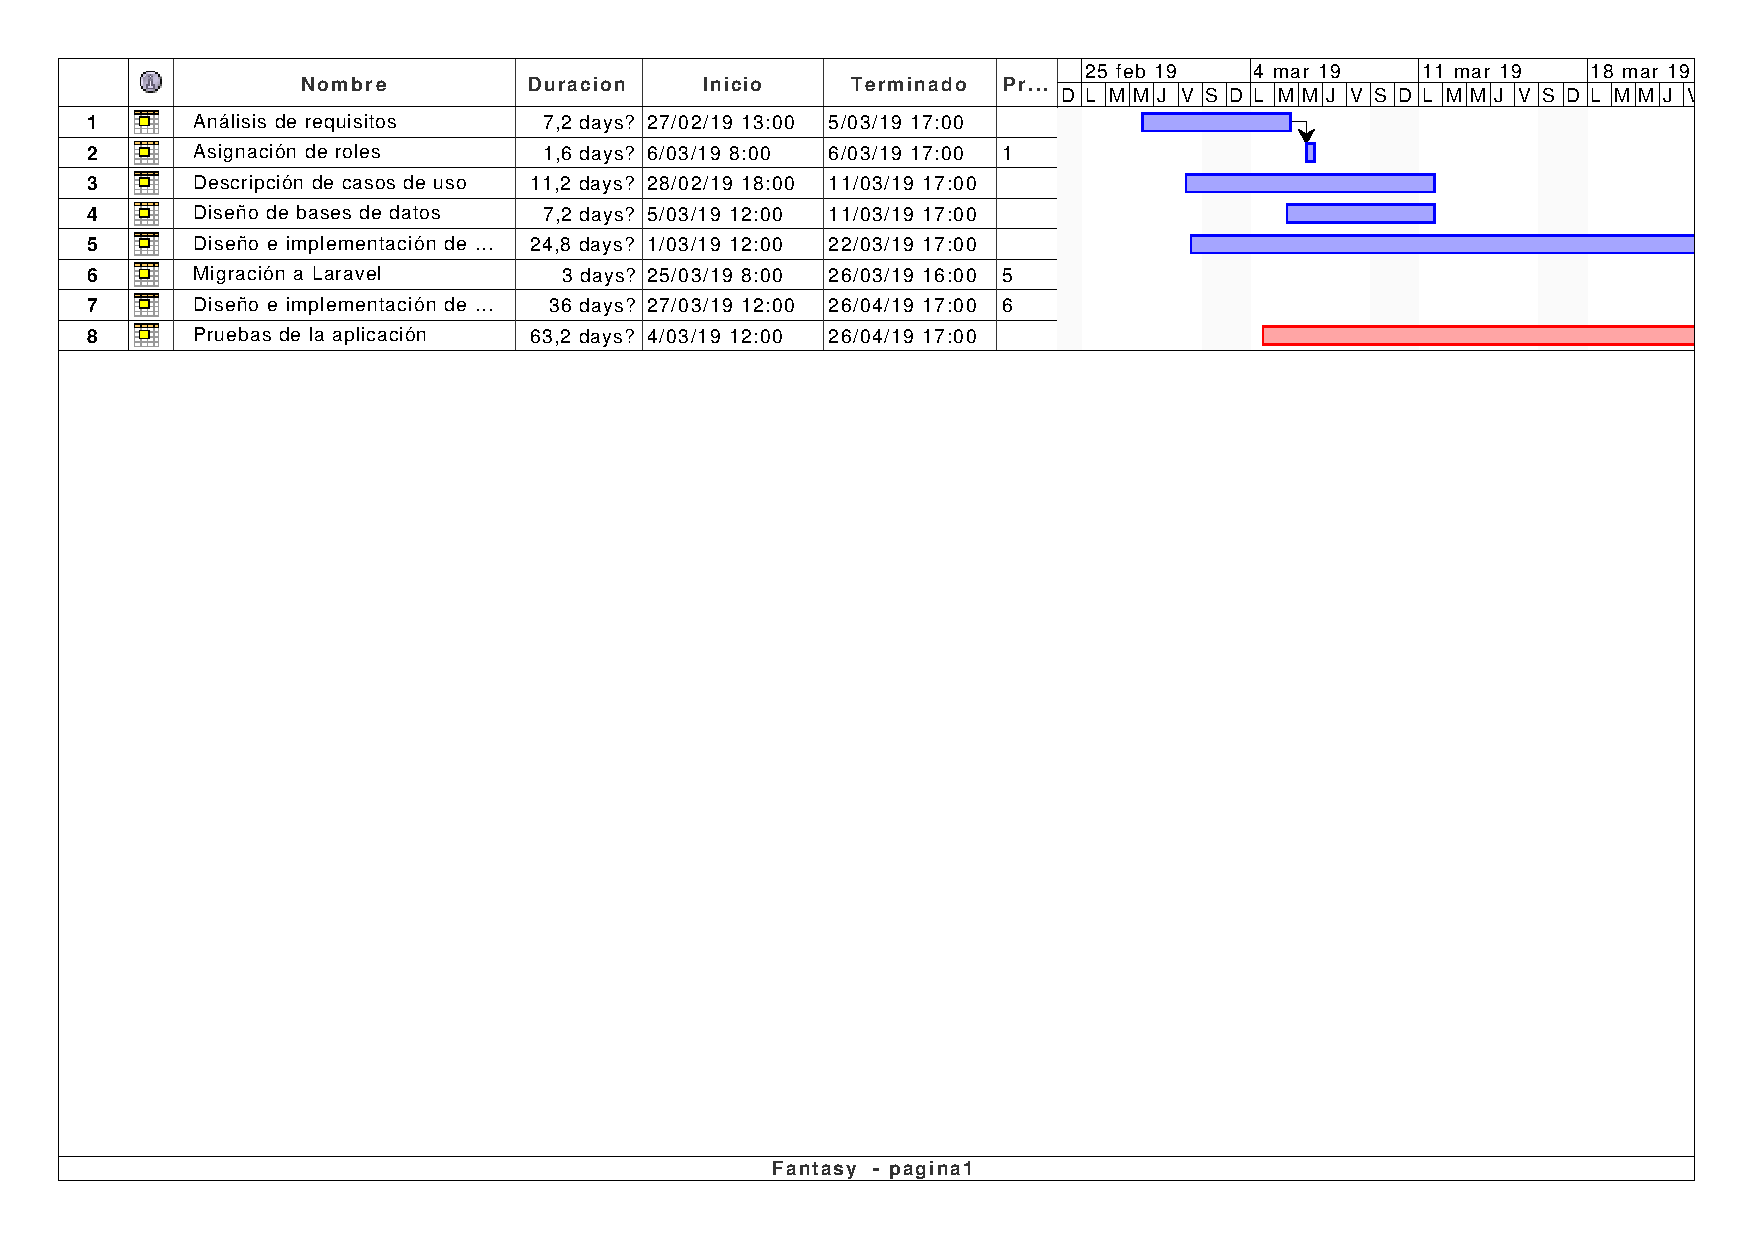
\includepdf[pages=-]{Planificacion}

\subsection{Organización}
\subsubsection{Roles}
\begin{itemize}
	\item \textbf{Scrum master:} Luis Gutiérrez Flores.
	\item \textbf{Administrador de sistemas:} Alejandro José Caraballo García.
	\item \textbf{Producto owner:} Jesús Rodríguez Heras.
	\item \textbf{Analista:} Nicolás Ruiz Requejo.
	\item \textbf{Arquitecto Software:} Arantzazu Otal Alberro.
	\item \textbf{Desarrollador:} Todos.
	\item \textbf{Diseñador de interfaz de usuario:} Alejandro Segovia Gallardo.
	\item \textbf{Tester:} Gabriel Fernando Sánchez Reina.
\end{itemize}

\subsubsection{Recursos hardware y sofware}
Como recursos hardware tenemos los portátiles de los 7 miembros del grupo y el servidor de Stimey.

Como recursos software tenemos el framework Laravel, Atom, Visual Studio Code, TeXStudio, PhPMyAdmin, MySQL, GitHub.

\subsection{Costes}
\subsubsection{Costes humanos}
\begin{itemize}
	\item Horas en el aprendizaje de Laravel.
	\item Horas en formación de PHP y MySQL.
	\item Horas en formación de GitHub.
	\item Horas de documentación.
\end{itemize}

\subsubsection{Costes materiales}
\begin{itemize}
	\item Nuestros ordenadores.
	\item Transporte a la escuela.
	\item Gastos del servidor de Stimey.
\end{itemize}

\subsection{Gestión de riesgos}
\begin{itemize}
	\item No cumplir plazos por intentar abarcar demasiado y dejar funcionalidades incompletas.
\end{itemize}

\end{document}